% EBP course: session 11
% Last class
% Thomas Klee
% 17 Apr 2019

% Preamble
\documentclass{beamer}
\usetheme{Singapore}
\usefonttheme[onlysmall]{structurebold}
\setbeamerfont{title}{shape=\itshape,family=\rmfamily}
\usepackage{graphicx}
\usepackage[english]{babel}
\usepackage[utf8x]{inputenc}
\usepackage{amsfonts, amsmath, amsthm, amssymb} % for math fonts, symbols and environments
\usepackage{xcolor}
\usepackage{booktabs}
\usepackage{ctable} % for command-driven tables
\usepackage{wasysym}
\usepackage{marvosym}
\usepackage[natbibapa]{apacite}
\beamertemplatenavigationsymbolsempty % uncomment to add slide navigation symbols to each slide
\setbeamertemplate{footline}[frame number]
\usepackage{appendixnumberbeamer}  % to suppress page numbers on extra slides

\mode<presentation>

% information for title slide
\title{Communicating Your Findings in Writing}
\subtitle{}
\author{Evidence-Based Practice in Speech-Language Therapy \\ (SHSC 2033)}
\institute{Session 11}
\date{Thomas Klee \& Elizabeth Barrett}
\titlegraphic{
\includegraphics[width=6cm]{images/logo_CE_C.jpg}} % HKU logo

\begin{document}

% create title slide with information above
\begin{frame}
	\titlepage
\end{frame}

% 
\begin{frame}{Outline}
	\begin{enumerate}
	\item Course evaluation
	\item Writing and Written Assignment 2
	\item Your questions
	\end {enumerate}
\end{frame}

\section{Course evaluation}

% 
\begin{frame}{Course evaluation}
	\begin{itemize}
	\item[\RIGHTarrow] Please let us know what you thought about the course.  
	\item[\RIGHTarrow] It's important.
	\item[\RIGHTarrow] We listen and take your feedback seriously.
	\end{itemize}
\end{frame}

\section{Writing}

\begin{frame}
	\begin{center}
	\Huge{Writing}
	\end{center}
\end{frame}

% 
\begin{frame}{Reminder from the first lecture\dots}
The REALLY BIG CHALLENGES \\
	\begin{itemize}
	\item Recognise that we all have biases that influence how we think.
	\item Be open to changing what you think when you encounter new (high quality) evidence.\footnote{Review slides 13 and 14 in Session 9 for a model.}
	\end{itemize}
\end{frame}

% 
\begin{frame}{Reasons for writing}
	\begin{enumerate}
	\item To \alert{learn}
	\item To \alert{communicate} to others
	\end{enumerate}
\end{frame}

% 
\begin{frame}{Improving your writing skills}
	\begin{center}
	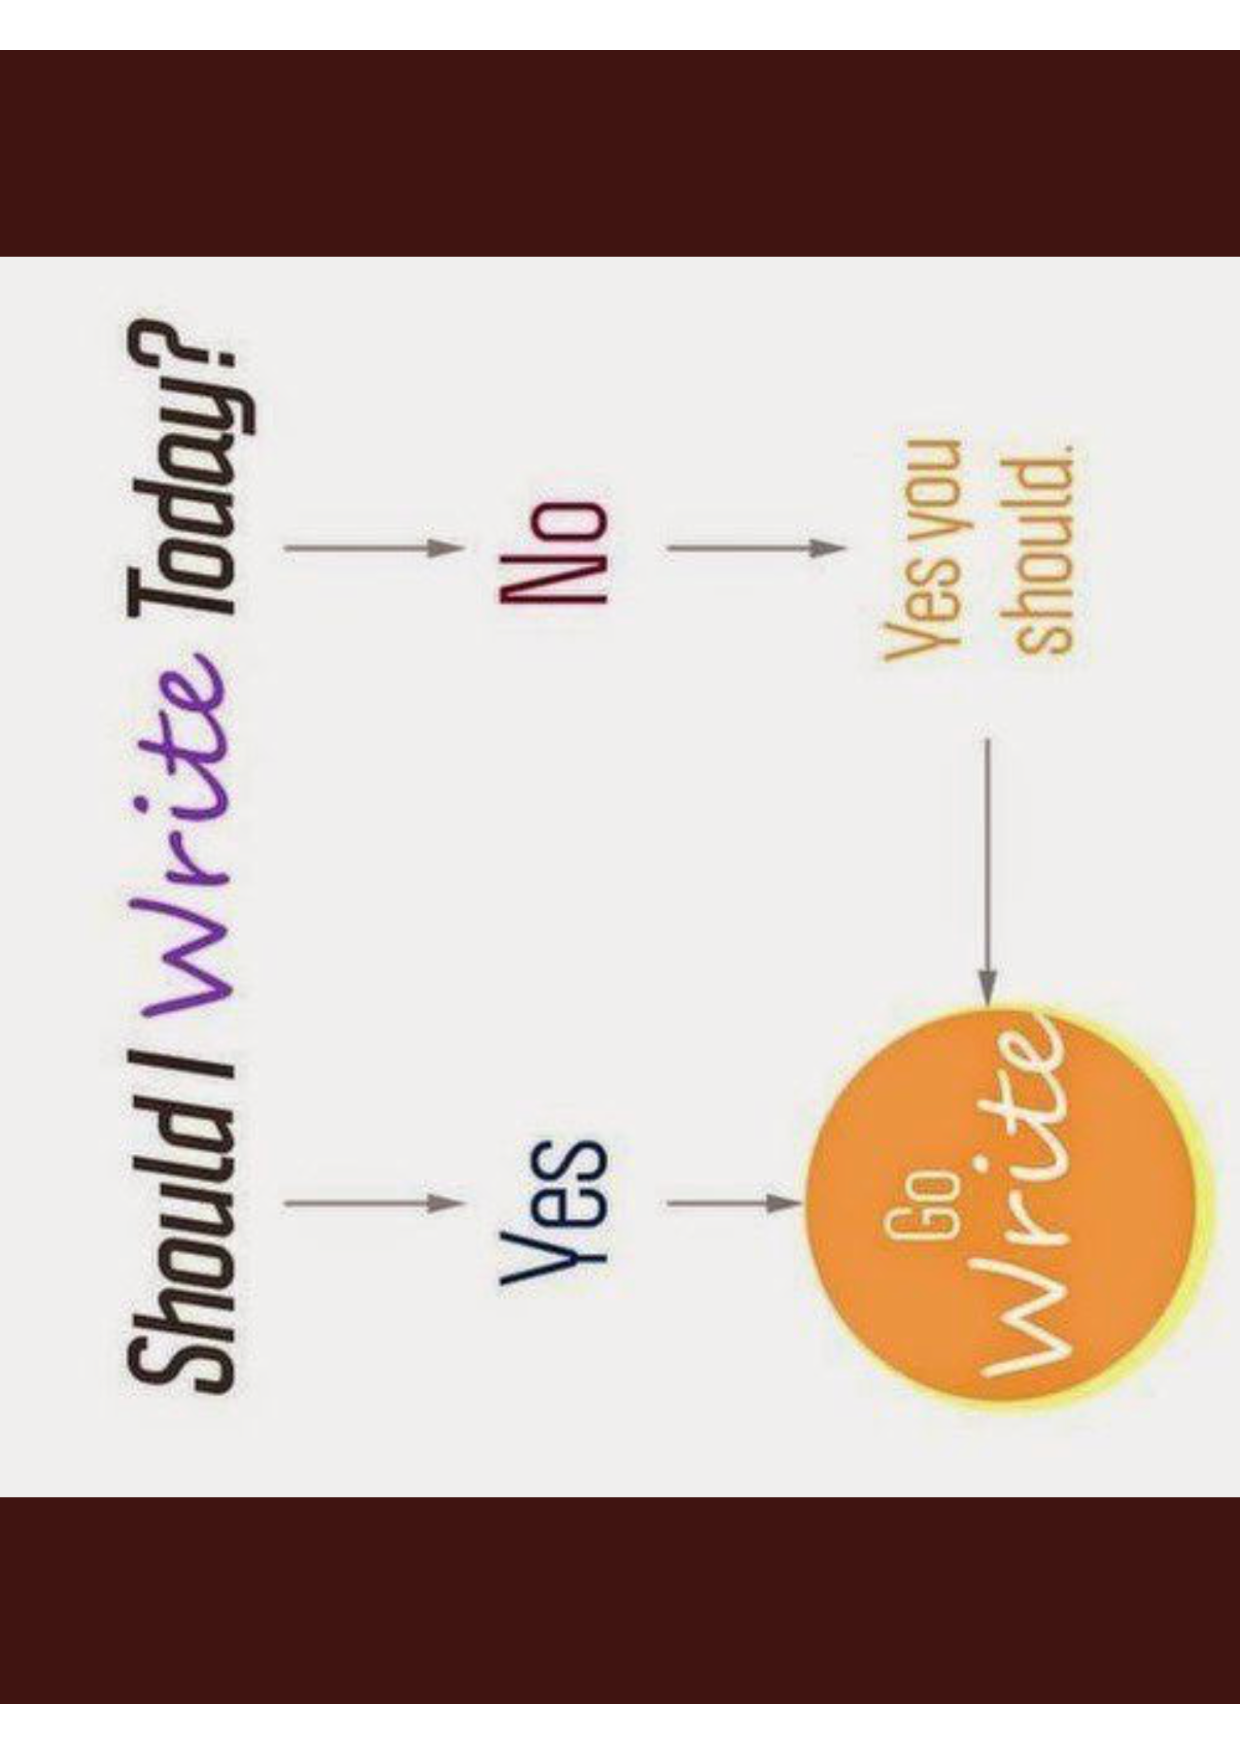
\includegraphics[angle = 270, width = .85\textwidth]{images/should_I_write_today.pdf}
	\end{center}
	\nocite{}
\end{frame}

% 
\begin{frame}{Common misspellings}
	\begin{center}
	\huge{\texttt{researches} \\
	\vspace{0.2in}
	\texttt{evidences} \\
	\vspace{0.2in}
	\texttt{literatures} \\
	\vspace{0.2in}
	\texttt{informations}
	}
	\end{center}
\end{frame}

% 
\begin{frame}{Recommended}
	\begin{center}
	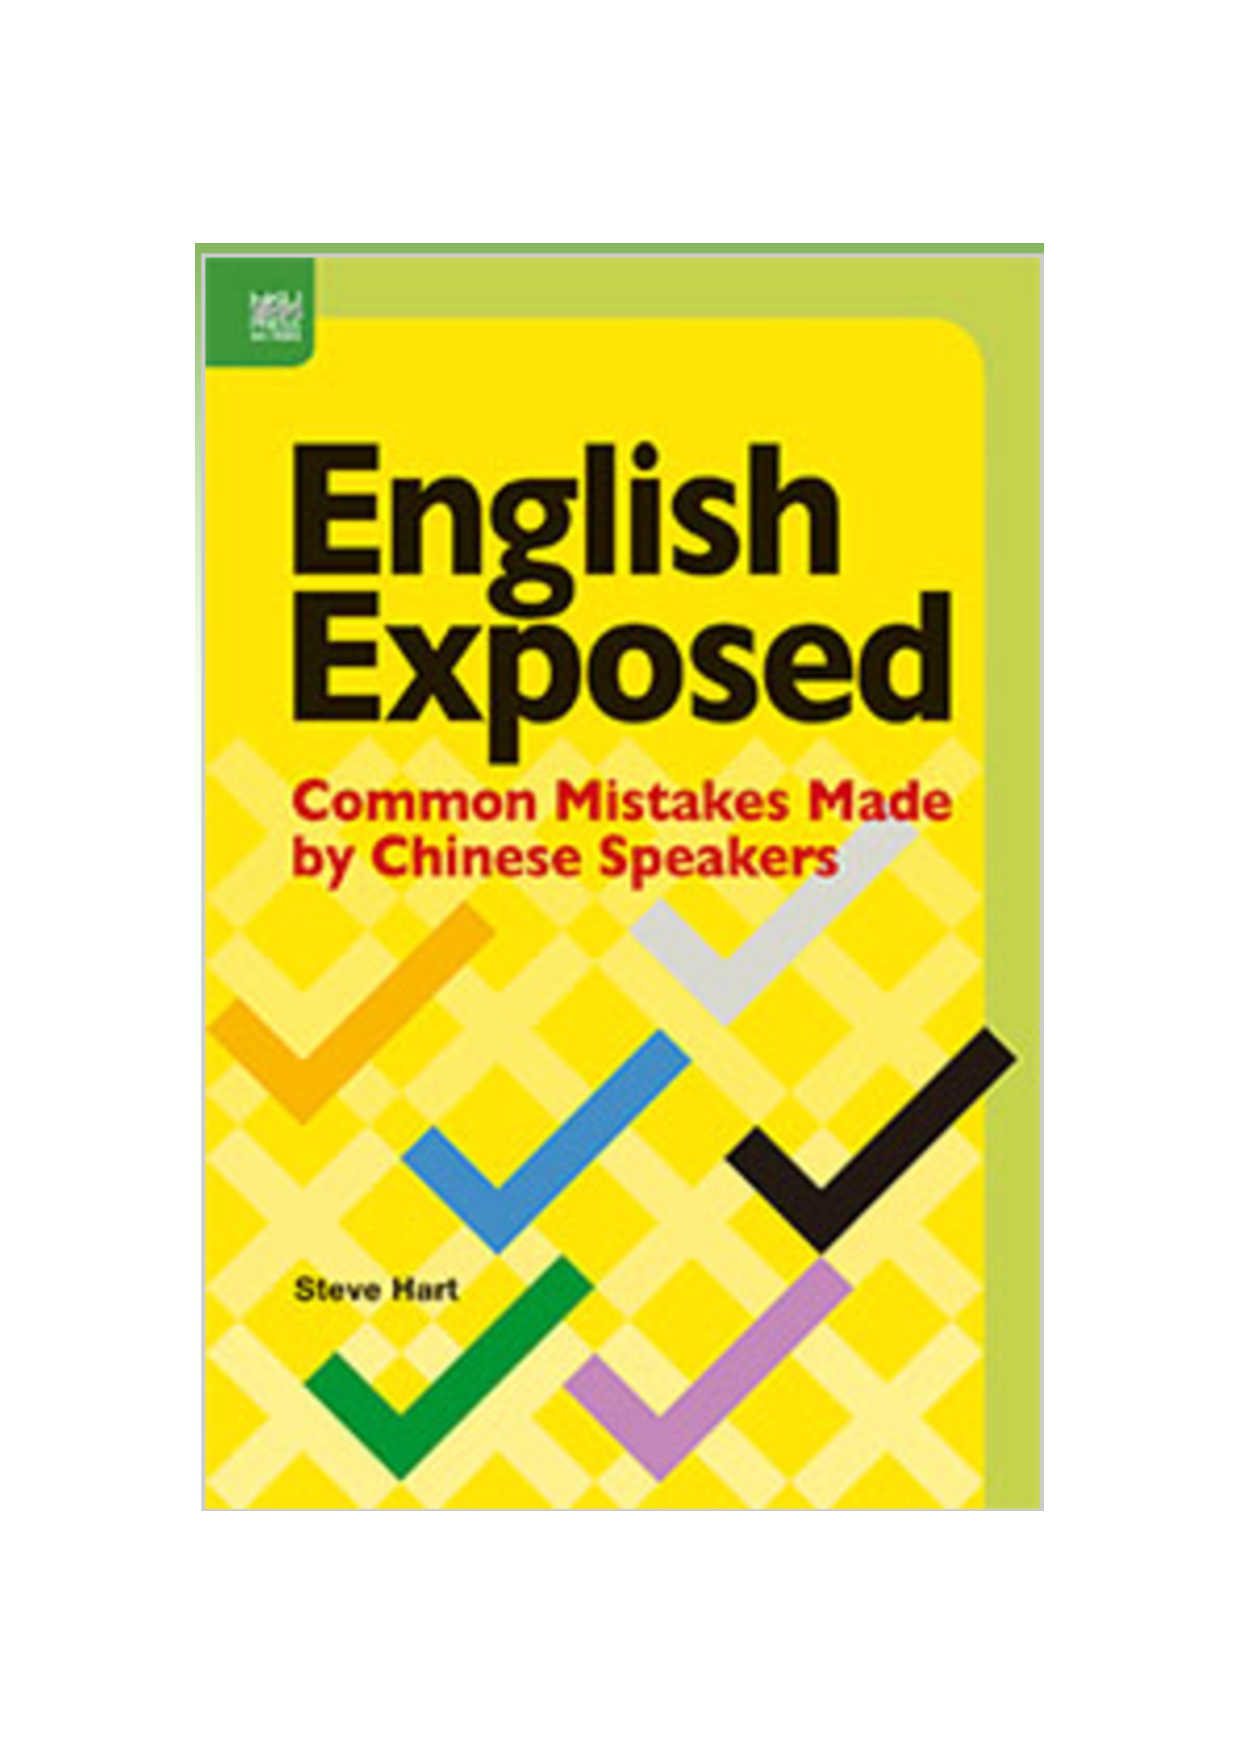
\includegraphics[width=.55\textwidth]{images/hart_book_cover.pdf}
	\end{center}
	\nocite{Hart2017}
\end{frame}


% 
\begin{frame}{Written assignment 2}
	\begin{enumerate}
	\item Your (revised) PICO question
	\item Rationale for asking your question
	\item Search strategy (databases searched; search terms used)
	\item How you decided which studies to include in your review and which to exclude
	\item Table of included studies based on Cochrane framework; see cochrane\_tables.pdf in \alert{Moodle: Resources} section
	\end{enumerate}
\end{frame}

% 
\begin{frame}{Written assignment 2}
	\begin{enumerate}
	\item[6.] Summary of the evidence you've critically appraised, \alert{followed by your conclusions}. Reflect on the PICO question you asked and whether it can be answered given the evidence you summarised.
	\item[7.] Suggestion(s) for future research addressing your question
	\item[8.] Reference list of included studies in APA format
	\item[9.] Critical appraisal checklists should \alert{not} be submitted.
	\item [10.] Submit your assignment to Turnitin on Moodle and put a printed copy in the Assignment Box (MW 742) by the deadline.
	\end{enumerate} 
\end{frame}

% 
\begin{frame}{\Pointinghand \hspace{0.05cm} Remember}
	\begin{itemize}
	\item[\checked] Put your student ID in the header or footer of each page. To enable anonymous marking, do \alert{not} identify yourself by name.
	\item[\checked] \alert{Maximum} of 6 double-spaced pages, \alert{plus} Cochrane table and references (not included in 6-page limit).
	\item[\checked] We stop reading after the page limit and base your mark on what you've written up to that point.	
	\end{itemize}
\end{frame}

% 
\begin{frame}{\Pointinghand \hspace{0.05cm} Remember}
	\begin{itemize}
	\item[\checked] All citations and references should conform to APA Publication Manual \citep{AmericanPsychologicalAssociation2010}.\footnote{See other writing resources in slides for session 2.}
	\item[\checked] All other formatting should conform to the APA Publication Manual, \alert{including font size and margins}.\footnote{We see many APA formatting errors in students' assignments; don't be one of those students!}
	\item[\checked] All words should be correctly spelled. Use a spell-checker.
	\end{itemize}
\end{frame}

\section{Q \& A}

% 
\begin{frame}{Q \& A}
	\begin{center}
	\dots about EBP \\
	\vspace{0.2in}
	\dots about the assignment
	\end{center}
\end{frame}

%
\begin{frame}%[shrink=15] % to reduce font size of references
	\frametitle{References}
	\bibliographystyle{apacite}
	\small\bibliography{/Users/thomasklee/Documents/Bibtex/library}
\end{frame}

\end{document}